%%%%%%%%%%%%%%%%%%%%%%%%%%%%%%%%%%%%%%%%%%%%%%%%%%%%%%%%%%%%%%%
%%  Versão final do IEEExplore
%%%%%%%%%%%%%%%%%%%%%%%%%%%%%%%%%%%%%%%%%%%%%%%%%%%%%%%%%%%%%%%

%\documentclass[10pt, conference, compsocconf]{IEEEtran}
\documentclass[a4paper]{sbgames}               

\usepackage{times}
\usepackage{graphicx}
\usepackage{amsmath,amssymb,amsthm,siunitx}
\usepackage[brazil,american]{babel}
\usepackage[utf8]{inputenc}

%% use this for zero \parindent and non-zero \parskip, intelligently.
\usepackage{parskip}

%% the 'caption' package provides a nicer-looking replacement
%\usepackage[labelfont=bf,textfont=it]{caption}

\usepackage{url}

\begin{document}

%% Paper title.
\title{Título do Artigo}


% \author{\IEEEauthorblockN{Autor1, Autor2, and Autor3}
% \IEEEauthorblockA{Dept. of Computer Science\\
% University of Brasilia\\ Brasilia, Brazil\\
% Email: \{autor1, autor2\}@gmail.com autor3@hotmail.com}
% }

 \author{ Autor1 
         \hspace{28pt} Autor2 \\
         \vspace{0pt} \\
         {University of Brasília, Dept. of Computer Science, Brazil} }
        
 \contactinfo{autor1@gmail.com \\ autor2@hotmail.br }



%\teaser{
%  \includegraphics[width=\linewidth]{sample.pdf}
%  (a)\hspace{150pt} (b) \hspace{150pt}   (c)
%  \caption{(a) Guitar Hero III screen; (b) DE2-35 Kit on top of PlayStation 2; (c) Grybot}
%  \label{fig:01}
%}


% make the title area
\maketitle

% Abstract section.
\begin{abstract}
Escreva aqui um resumo do projeto.
Este trabalho apresenta o desenvolvimento de ....
Lorem ipsum dolor sit amet, consectetur adipiscing elit, sed do eiusmod tempor incididunt ut labore et dolore magna aliqua. Ut enim ad minim veniam, quis nostrud exercitation ullamco laboris nisi ut aliquip ex ea commodo consequat. Duis aute irure dolor in reprehenderit in voluptate velit esse cillum dolore eu fugiat nulla pariatur. Excepteur sint occaecat cupidatat non proident, sunt in culpa qui officia deserunt mollit anim id est laborum

\end{abstract}

%% Keywords that describe your work.
\keywords{Robot, Guitar Hero, FPGA, Artificial Intelligence}
% \begin{IEEEkeywords}
% Jogos; Processador MIPS; FPGA;
% \end{IEEEkeywords}


\section{Introdução}
\label{sec:introducao}

Jogos digitais tem sido amplamente usados para...

Lorem ipsum dolor sit amet, consectetur adipiscing elit. Ut at dapibus arcu, id semper enim. Duis at dui pharetra, luctus lectus a, consectetur arcu. Maecenas lacinia tristique nisl sed rhoncus. Integer et sem eros. Phasellus tempor dapibus augue quis lacinia. Quisque leo justo, porta ac porttitor sed, consequat ut dui. Cras commodo mollis sagittis. Quisque maximus odio at leo ornare, sed malesuada augue dictum. Nunc vitae feugiat nisi, in aliquam nisi. Nullam dictum, nibh nec ornare faucibus, sapien nibh pulvinar mauris, ut maximus eros dolor quis nunc.

Este trabalho apresenta ...

Lorem ipsum dolor sit amet, consectetur adipiscing elit. Suspendisse condimentum id erat nec bibendum. Proin placerat arcu sed cursus viverra. Lorem ipsum dolor sit amet, consectetur adipiscing elit. Aenean venenatis, est a porta lobortis, ligula ante ultrices ligula, eget porta purus elit eu justo. Suspendisse fringilla efficitur tortor, ac sollicitudin erat fringilla quis. In hac habitasse platea dictumst. Pellentesque placerat erat sed orci malesuada ultrices. Praesent vulputate tellus risus, at suscipit neque volutpat in. Duis volutpat mattis lacus, vel gravida est. Nulla tincidunt interdum auctor. Etiam non viverra est.


\begin{figure}[htb]
  \begin{center}
   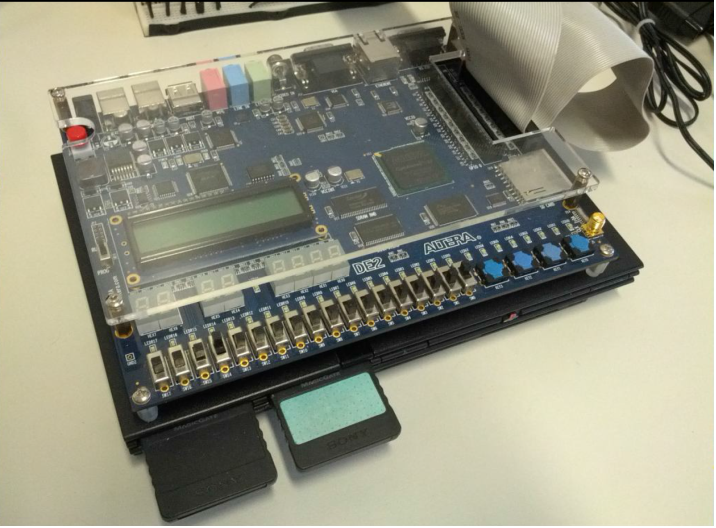
\includegraphics[width=1.0\linewidth]{./Figures/Fig1b.png}
  \end{center}
  \caption{O que é a figura}
  \label{fig:01}
\end{figure}

A Figura \ref{fig:01} mostra o kit de desenvolvimento DE2-70  ~\cite{Alt}.

Lorem ipsum dolor sit amet, consectetur adipiscing elit, sed do eiusmod tempor incididunt ut labore et dolore magna aliqua. Ut enim ad minim veniam, quis nostrud exercitation ullamco laboris nisi ut aliquip ex ea commodo consequat. Duis aute irure dolor in reprehenderit in voluptate velit esse cillum dolore eu fugiat nulla pariatur. Excepteur sint occaecat cupidatat non proident, sunt in culpa qui officia deserunt mollit anim id est laborum.

Na seção \ref{sec:Metodologia} será apresentada a metodologia utilizada. A seção \ref{sec:Resultados} apresenta os resultados obtidos. A seção \ref{sec:Conclusao} conclui este trabalho.

\section{Metodologia}
\label{sec:Metodologia}

Apresentar aqui como o projeto foi desenvolvido e quais as ferramentas usadas.

Lorem ipsum dolor sit amet, consectetur adipiscing elit, sed do eiusmod tempor incididunt ut labore et dolore magna aliqua. Ut enim ad minim veniam, quis nostrud exercitation ullamco laboris nisi ut aliquip ex ea commodo consequat. Duis aute irure dolor in reprehenderit in voluptate velit esse cillum dolore eu fugiat nulla pariatur. Excepteur sint occaecat cupidatat non proident, sunt in culpa qui officia deserunt mollit anim id est laborum.



\subsection{Arquitetura MIPS}{
\label{sec:MIPS}
Exemplo de subseção. A arquitetura MIPS \cite{patterson2005organizaccao} foi desenvolvida por ....


Lorem ipsum dolor sit amet, consectetur adipiscing elit. Aenean nec magna lectus. Donec egestas risus quis mollis venenatis. Nullam vel tellus enim. Aliquam erat volutpat. Phasellus a urna et tellus venenatis aliquet. Integer sit amet condimentum leo. Etiam massa nisi, rhoncus eget condimentum pharetra, imperdiet vitae eros. Nunc porta nisi facilisis, feugiat odio sit amet, ullamcorper tortor. Cras et urna cursus, mollis nibh quis, blandit risus.

Pellentesque tincidunt ultrices ex at varius. Pellentesque sit amet sapien in enim vehicula tincidunt vel ac augue. Integer ultricies vulputate massa at scelerisque. Curabitur ut quam porttitor, rhoncus felis eget, semper sapien. Integer accumsan nisi et leo suscipit iaculis. Suspendisse potenti. Class aptent taciti sociosqu ad litora torquent per conubia nostra, per inceptos himenaeos. Aenean pretium lacus sed quam volutpat congue. Ut sapien erat, dictum nec faucibus vel, finibus tempor nisl. 
}


\subsection{Simulador/Montador MARS}{
\label{sec:Mars}
Exemplo de subseção. O Mars \textit{MIPS Assembler and Runtime Simulator} \cite{Mars1} é um simulador desenvolvido por...

Lorem ipsum dolor sit amet, consectetur adipiscing elit. Aenean nec magna lectus. Donec egestas risus quis mollis venenatis. Nullam vel tellus enim. Aliquam erat volutpat. Phasellus a urna et tellus venenatis aliquet. Integer sit amet condimentum leo. Etiam massa nisi, rhoncus eget condimentum pharetra, imperdiet vitae eros. Nunc porta nisi facilisis, feugiat odio sit amet, ullamcorper tortor. Cras et urna cursus, mollis nibh quis, blandit risus.

Pellentesque tincidunt ultrices ex at varius. Pellentesque sit amet sapien in enim vehicula tincidunt vel ac augue. Integer ultricies vulputate massa at scelerisque. Curabitur ut quam porttitor, rhoncus felis eget, semper sapien. Integer accumsan nisi et leo suscipit iaculis. Suspendisse potenti. Class aptent taciti sociosqu ad litora torquent per conubia nostra, per inceptos himenaeos. Aenean pretium lacus sed quam volutpat congue. Ut sapien erat, dictum nec faucibus vel, finibus tempor nisl. 
}


\section{Resultados Obtidos}
\label{sec:Resultados}
Apresentar aqui os resultados obtidos, telas e link para vídeos e comentários.



Lorem ipsum dolor sit amet, consectetur adipiscing elit. Nunc eu mi cursus, pretium lectus vel, commodo neque. Nulla facilisi. Duis in quam non metus lobortis sagittis. Nunc ac auctor mi. Nullam imperdiet orci eget neque accumsan, eget ornare turpis cursus. Sed ut cursus sapien, vel accumsan neque. Donec dignissim maximus sapien non commodo. Praesent a gravida metus. Duis eget nulla luctus, finibus ex sed, ornare velit. Pellentesque habitant morbi tristique senectus et netus et malesuada fames ac turpis egestas. Curabitur placerat efficitur velit, eget auctor eros posuere nec. Morbi pretium purus in libero porttitor interdum.

Ut convallis egestas libero, sit amet tempor sem volutpat pretium. Nam ut libero mattis, interdum purus sit amet, fermentum diam. Integer a mi iaculis, egestas risus in, tempus eros. Donec elementum aliquet ante, nec ultrices lectus iaculis id. Integer pretium, mi id tempor blandit, elit sem viverra mi, sit amet rhoncus nunc sapien et mi. Etiam egestas at nisl non finibus. Mauris interdum elit lorem, sit amet eleifend ex rhoncus ultrices. Donec vulputate leo et velit viverra, sit amet volutpat nulla aliquam. Aenean quis velit sed arcu dapibus sagittis.

Etiam magna ipsum, eleifend ut egestas ac, varius ac mauris. Praesent non nisl vitae dui fermentum fermentum. Fusce a tortor vitae lorem semper scelerisque sagittis et magna. Aenean tincidunt, lacus nec lacinia tempus, felis urna placerat orci, at facilisis urna quam in nibh. Nam sagittis facilisis libero, non scelerisque leo finibus ac. Nulla neque purus, viverra sit amet elementum vel, iaculis in dui. Praesent sit amet condimentum est. Proin convallis sapien sed semper interdum. Mauris semper laoreet elementum. Nam eu fringilla odio, a rhoncus sapien. Etiam id sem quis sapien bibendum porttitor. Etiam eu luctus odio. Aenean vel imperdiet est, et dignissim mauris. Donec quam massa, accumsan eget tellus quis, accumsan dignissim enim. 

\section{Conclusão}
\label{sec:Conclusao}
Este trabalho apresentou...

Lorem ipsum dolor sit amet, consectetur adipiscing elit. Nunc eu mi cursus, pretium lectus vel, commodo neque. Nulla facilisi. Duis in quam non metus lobortis sagittis. Nunc ac auctor mi. Nullam imperdiet orci eget neque accumsan, eget ornare turpis cursus. Sed ut cursus sapien, vel accumsan neque. Donec dignissim maximus sapien non commodo. Praesent a gravida metus. Duis eget nulla luctus, finibus ex sed, ornare velit. Pellentesque habitant morbi tristique senectus et netus et malesuada fames ac turpis egestas. Curabitur placerat efficitur velit, eget auctor eros posuere nec. Morbi pretium purus in libero porttitor interdum.

%{\bf Acknowledgments}
%[Blind Review]

%\newcommand{\BIBdecl}{\setlength{\itemsep}{-0.5 em}}
%\bibliographystyle{IEEEtran}
\bibliographystyle{sbgames}
\bibliography{bibliography}

\end{document}
